\section{Preliminary results}

OLS fitted 12 predictors (n=51,341). Evidence that adjusted weekend--weekday contrasts differ by room type is insufficient (95\% CI \ensuremath{-}7.33 to 15.09; p=0.497).

\begin{table}[!htbp]
\centering
\caption{All coefficients (SEs), EUR. References: Amsterdam, weekdays, private rooms, non-Superhosts, single offers.}
\label{tab:coefficients}
\small
\setlength{\tabcolsep}{5pt}
\renewcommand{\arraystretch}{1.14}
\begin{tabularx}{\linewidth}{@{}Xrrr@{}}
\toprule
\textbf{Term / city} & \textbf{Estimate (SE)} & \shortstack[r]{\textbf{City $\times$}\\\textbf{weekend (SE)}} & \shortstack[r]{\textbf{City $\times$}\\\textbf{entire (SE)}} \\
\midrule
Intercept & \ensuremath{-}12.34 (18.89) &  &  \\
\var{day_type}: weekends & 26.00 (12.92) &  &  \\
\var{room_type}: entire home/apt & 285.87 (12.93) &  &  \\
\var{person_capacity} & 27.80 (1.40) &  &  \\
\var{bedrooms} & 81.00 (2.51) &  &  \\
\var{cleanliness_rating} & 5.76 (1.90) &  &  \\
\var{guest_satisfaction_overall} & 0.93 (0.21) &  &  \\
\var{host_is_superhost}: Superhost & 4.96 (3.06) &  &  \\
\var{dist} & \ensuremath{-}0.36 (0.94) &  &  \\
\var{metro_dist} & \ensuremath{-}4.95 (1.88) &  &  \\
\var{attr_index_norm} & 6.58 (0.20) &  &  \\
\var{host_portfolio}: 2--4 offers & 8.47 (3.23) &  &  \\
\var{host_portfolio}: 5+ offers & 25.09 (3.28) &  &  \\
\var{day_type} \(\times\) \var{room_type} & 3.88 (5.72) &  &  \\
\midrule
Athens & \ensuremath{-}216.28 (18.34) & \ensuremath{-}34.45 (14.91) & \ensuremath{-}302.27 (19.46) \\
Barcelona & \ensuremath{-}192.49 (13.23) & 19.09 (16.67) & 0.29 (18.67) \\
Berlin & \ensuremath{-}207.25 (14.25) & \ensuremath{-}10.78 (17.06) & \ensuremath{-}170.74 (17.43) \\
Budapest & \ensuremath{-}250.31 (17.98) & \ensuremath{-}7.86 (15.52) & \ensuremath{-}279.88 (19.35) \\
Lisbon & \ensuremath{-}180.26 (13.32) & \ensuremath{-}20.68 (14.62) & \ensuremath{-}238.46 (15.05) \\
London & \ensuremath{-}175.93 (12.03) & \ensuremath{-}28.83 (13.78) & \ensuremath{-}50.85 (13.92) \\
Paris & \ensuremath{-}88.02 (13.44) & \ensuremath{-}46.35 (14.40) & \ensuremath{-}182.06 (15.13) \\
Rome & \ensuremath{-}198.85 (12.07) & \ensuremath{-}23.31 (13.88) & \ensuremath{-}280.35 (14.10) \\
Vienna & \ensuremath{-}142.72 (15.53) & \ensuremath{-}28.09 (15.80) & \ensuremath{-}277.50 (17.15) \\
\bottomrule
\end{tabularx}
\end{table}

The \texteuro{}81.00 bedroom slope and positive attraction association agree directionally with \citet{gyodi2021}. However, centre distance is inconclusive (p=0.702); differing controls may contribute.

\begin{itemize}[leftmargin=*,itemsep=2pt,topsep=4pt]
\item \textbf{Linearity:} Residual curvature suggests mean misspecification.
\item \textbf{Variance:} Rising scale-location suggests unequal variance.
\item \textbf{Error normality:} Q-Q upper tails depart from the reference line.
\item \textbf{Independence:} Unverified; nearby or repeated listings/hosts may be dependent.
\item \textbf{Conditional mean response:} Figure~\ref{fig:response} suggests one increasing trend; the condition remains unverified.
\item \textbf{Conditional mean predictors:} Curved attraction--distance trends (Figure~\ref{fig:pairs}) question conditional predictor linearity.
\item \textbf{Multicollinearity:} Full rank; some indicator VIFs \textgreater{}5 warrant caution.
\end{itemize}

Inference remains provisional; no repairs applied.

\begin{figure}[!htbp]
\centering
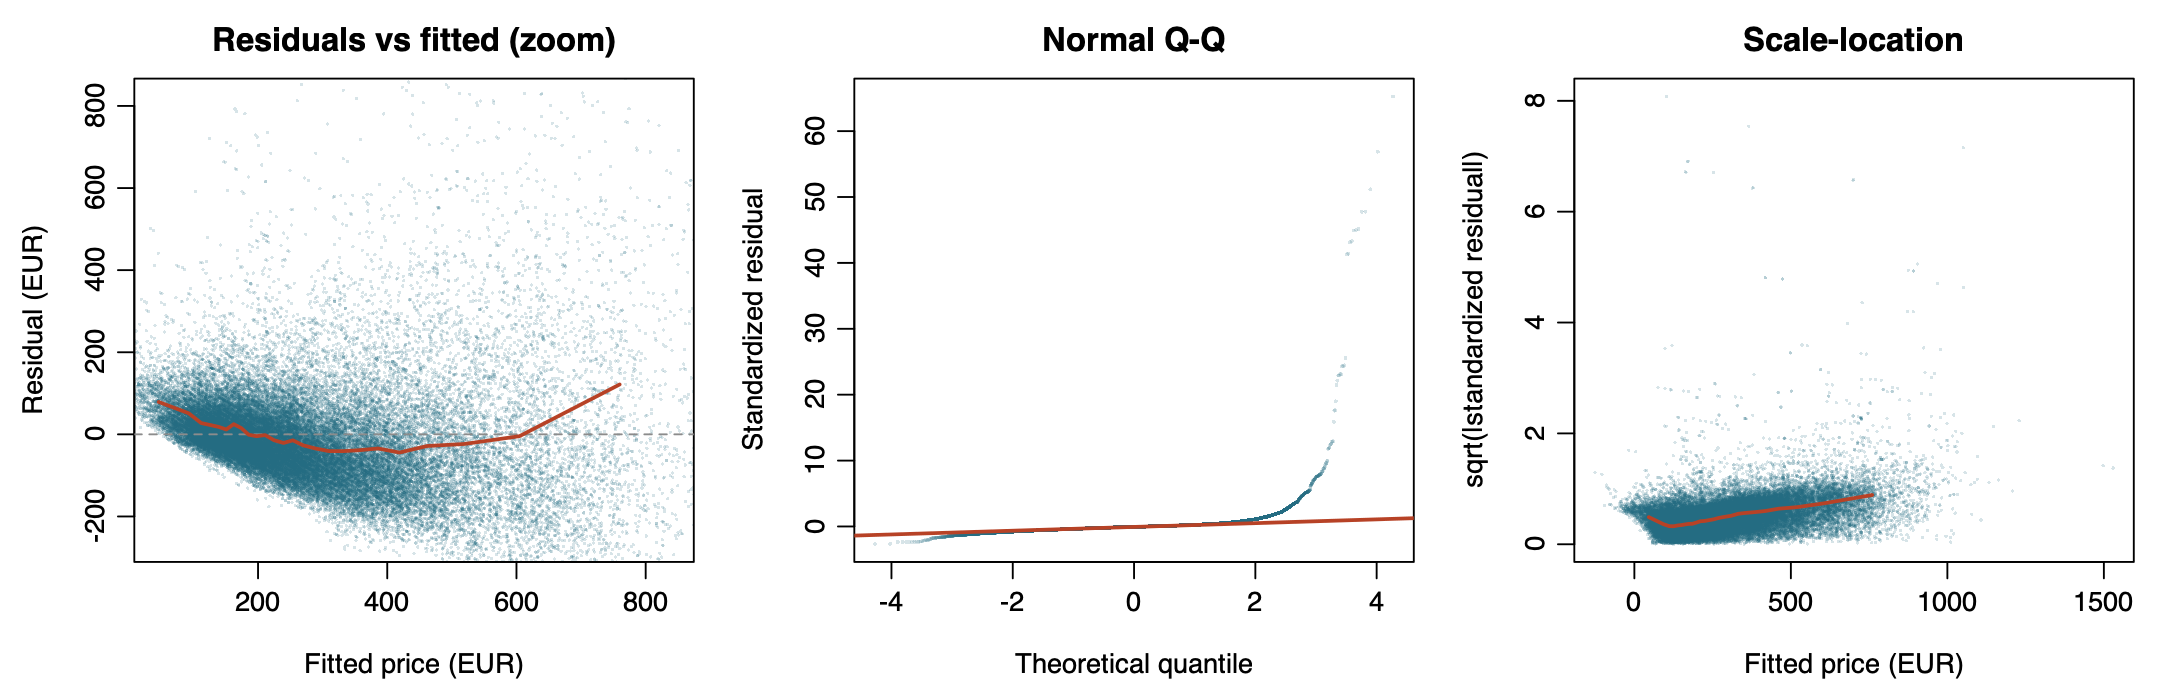
\includegraphics[width=1.00\linewidth]{figures/06_course_residual_diagnostics.png}
\caption{Residual diagnostics; left axes zoom central 99\%.}
\label{fig:diagnostics}
\end{figure}

\begin{figure}[!htbp]
\centering
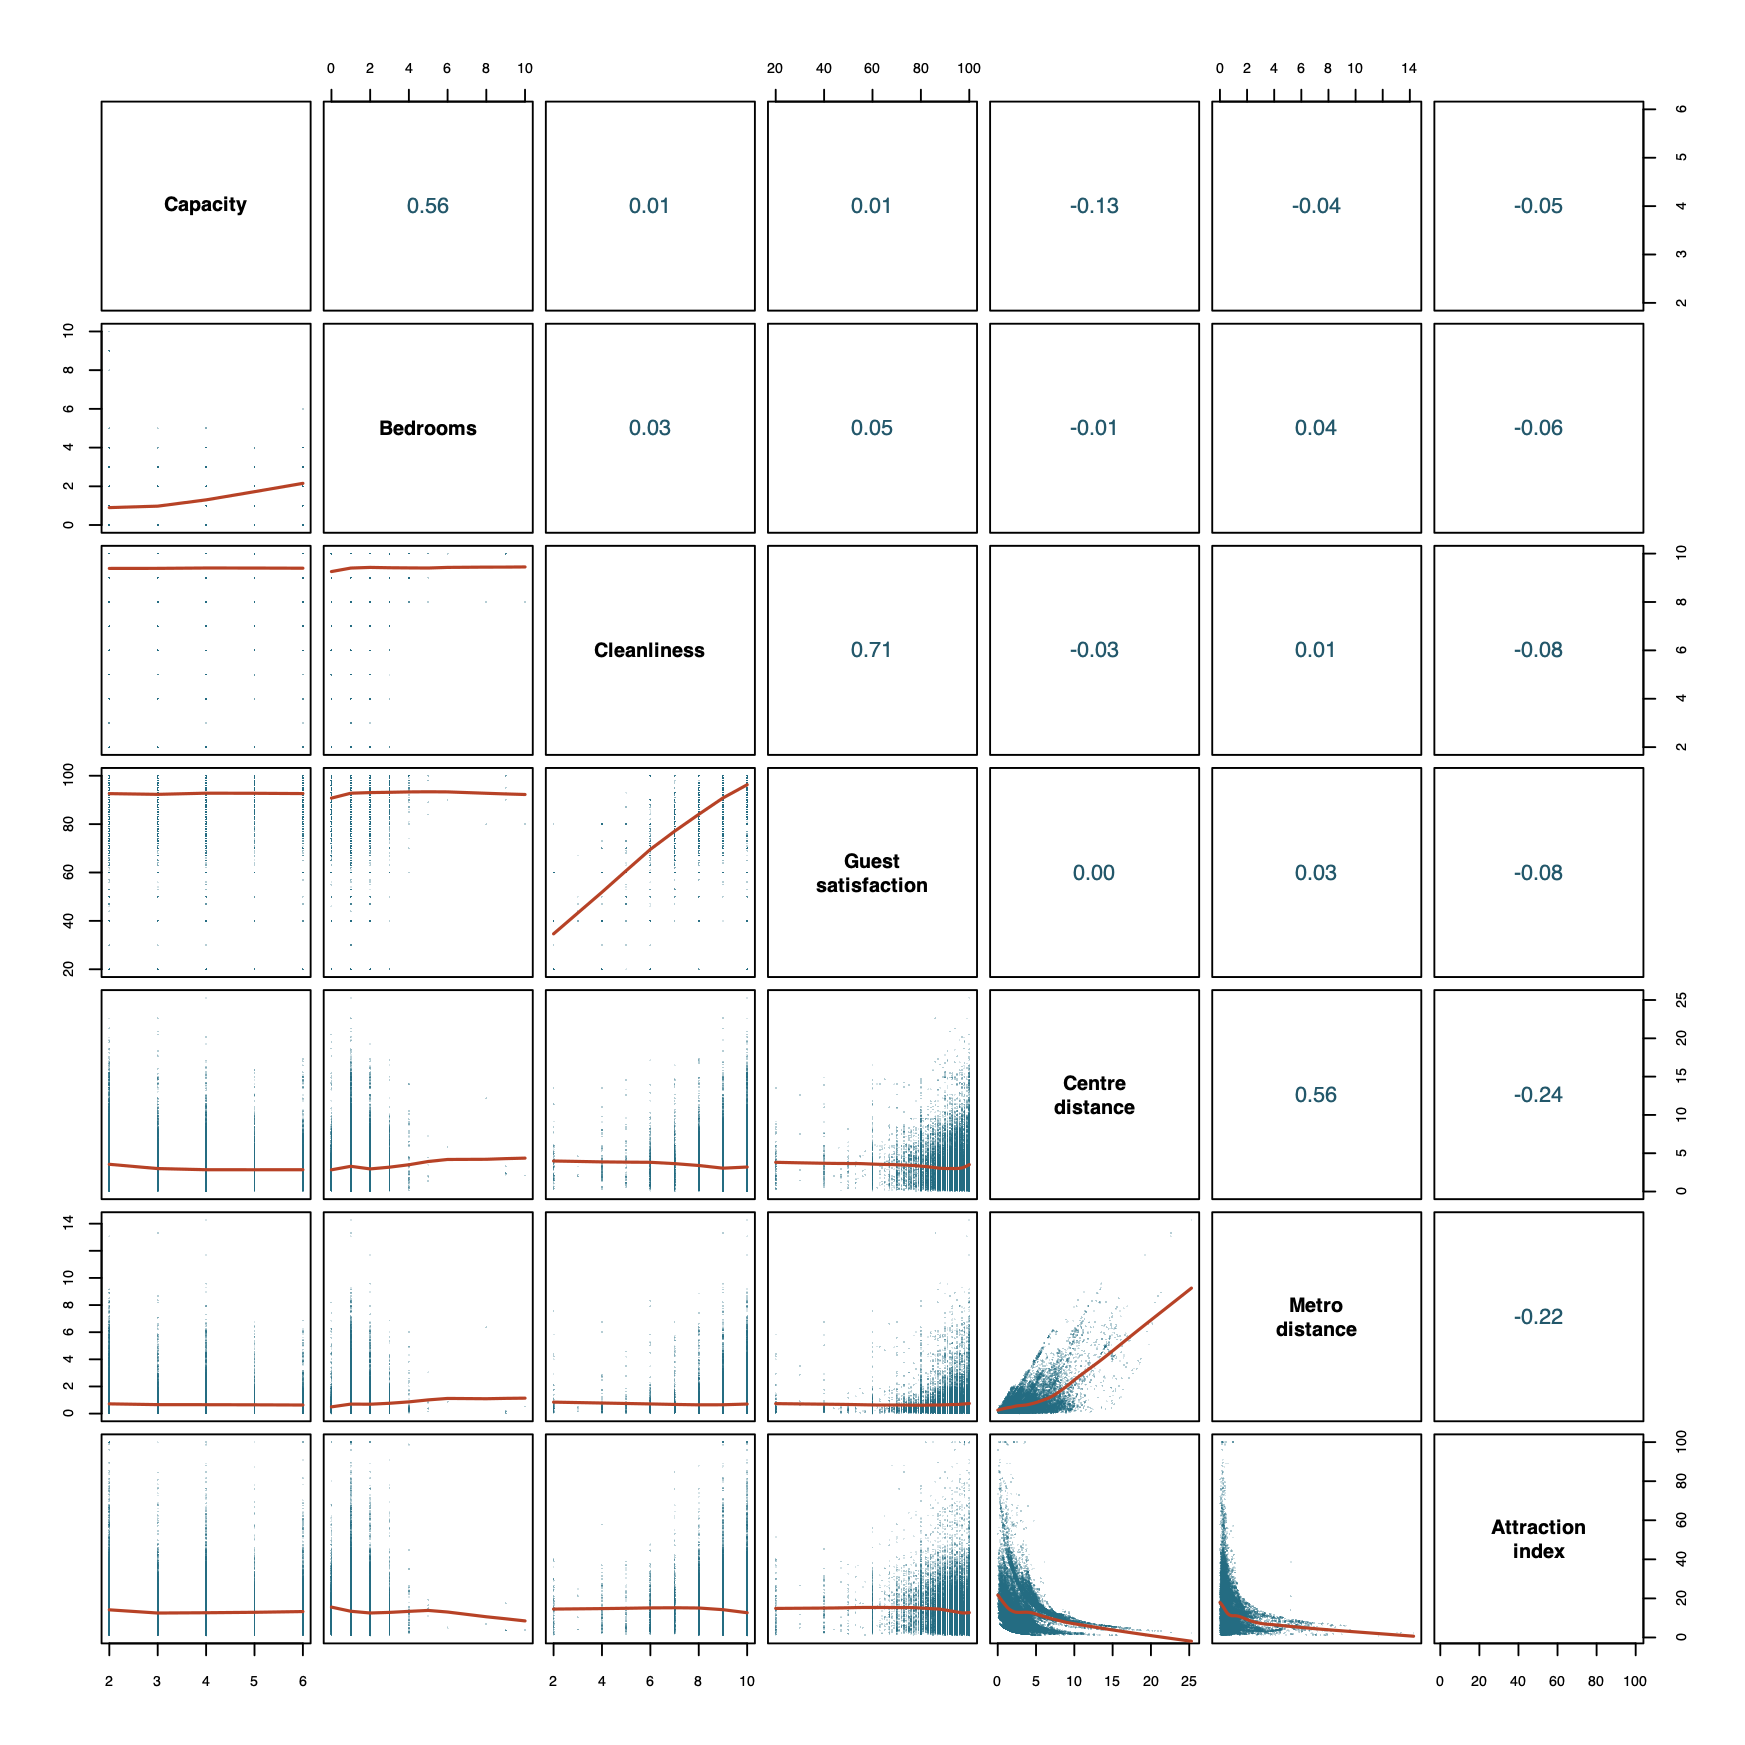
\includegraphics[width=0.96\linewidth]{figures/08_numeric_predictor_pairs.png}
\caption{Predictor pairs: smoothers below, Pearson correlations above.}
\label{fig:pairs}
\end{figure}

\begin{figure}[!htbp]
\centering
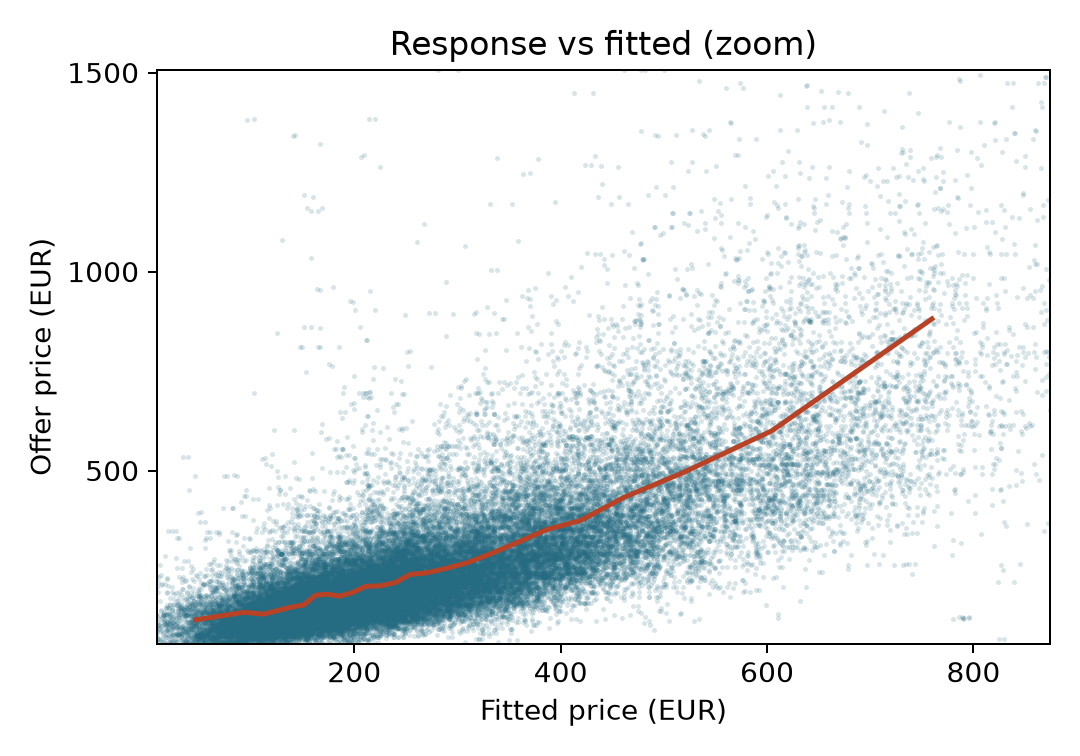
\includegraphics[width=0.70\linewidth]{figures/09_conditional_mean_response.png}
\caption{Response versus fitted: central 99\%; binned means.}
\label{fig:response}
\end{figure}

